\section{Game Server Features}

In addition to matchmaking, some features needed by the server during a match was also planned. In particular, we would like to be able to check whether or not a person is staying on his route. There are several interesting problems in performing such a check, including routes that are not straight lines, and geometry using latitude and longitude. The solution for these problems are described in this section.

\subsection{Decimal Degree Geometry}

When working with coordinates in the Google Maps \ac{API}, a position is denoted as a set of \texttt{(Longitude, Latitude)}, also known as decimal degrees, upon the surface of the earth. This poses two problems when calculating distances between two arbitrary points.

The first problem is that the earth is a sphere, which means that conventional Euclidean geometry will not be correct. However, since the server will have to do a lot of computations, we decided that 100\% precision was not required for this (for example, whether you are 22 meters or 23 meters off route does not really matter), we decided to convert points to an offset in meters from \texttt{(Longitude, Latitude)} = \texttt{(0, 0)}, and then use Euclidean geometry on the resulting points.

That leads to the second problem. One degree of longitude's length in meters varies depending on the latitude\cite{wikidecimaldegrees}. This meant a function, seen in \autoref{lst:sprint3-coord-offset}, had to be created to convert from coordinates in \texttt{(Longitude, Latitude)} to an \texttt{(x, y)} offset in meters. This approach resulted in very small imprecisions (on a scale of centimeters), though imprecisions grow as you get further from the equator.

\begin{lstlisting}[label={lst:sprint3-coord-offset},caption={Convert Decimal Degrees to Offset in Meters},language={Python}]
def metric_offset(self, coord):
	return (coord[0] * 111319.9 * cos(radians(coord[1])) , coord[1] * 111319.9)
\end{lstlisting}

\subsection{Distance Between Point and Route}

Finding the distance between two points is not enough to determine whether a point is close to a route. The first problem with this, is that there might be quite far between two waypoints on a route, that is a user might have a 5 kilometre long route with just two waypoints. The natural solution to this is to project the point onto the line between the points and find the distance between those. However, as seen in \autoref{fig:sprint3-bad-route} using the line between the waypoints is often not indicative of the actual route.

\begin{figure}[ht]
 \caption{Non-linear Route}
 \label{fig:sprint3-bad-route}
 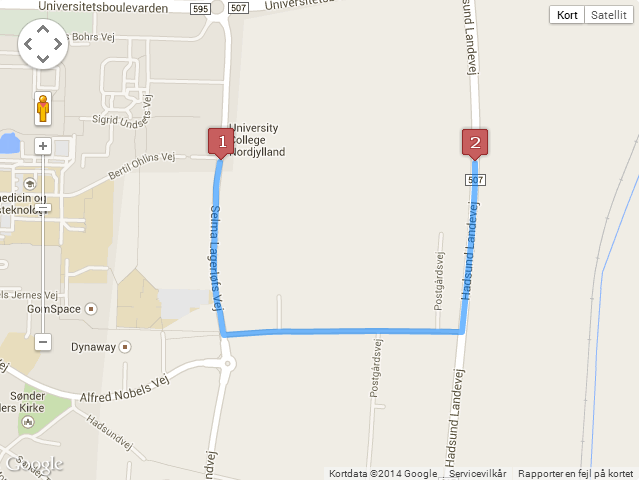
\includegraphics[scale=0.5]{img/sprint3br.png}
\end{figure}

\subsubsection{Decoding The Route}

The solution chosen to that problem, was to use drawn line from the Google Maps Directions Service as the route, instead of the waypoints. This line is known as a polyline, and is returned with every successful request to the directions service. As mentioned in \autoref{sec:sprint2-web}, the web server already sends a directions request for each route, so even though it is not being drawn anywhere, the server has access to this polyline. 

Additionally, the polyline retrieved from the map API is encoded as a string, which can easily be stored in the database, giving the game server access to the line without sending requests to the Google Maps \ac{API}. It is possible to decode this line into a series of points. We decided to do this using an existing piece of open source Python2 code\cite{decodepolyline}, which was ported to Python3. This function takes an encoded polyline and returns a list of \texttt{(Longitude, Latitude)} coordinates, which conveniently can be converted to the offsets we decided to work with, using the function seen in \autoref{lst:sprint3-coord-offset}.
